\section{Obnašanje ovc}

V tem poglavju si bomo ogledali dva modela obnašanja ovc avtorjev Str{\"o}mboma s sodelavci~\cite{Stroembom} in Ginellija s sodelavci~\cite{Ginelli}. Prvi model bomo nekoliko predelali in s tem naredili še tretji model. Za učenje in testiranje ovčarjev bomo uporabili ovce po vseh treh modelih in tako preverili robustnost metode vodenja za različne vrste agentov. Ovce so na začetku naključno enakomerno neodvisno porazdeljene v krog s polmerom 50~m na sredini kvadratnega pašnika s stranico dolgo 300~m. Na sredini ene stranice je 100~m širok vhod na cilj, ki mu bomo rekli staja. Psi ovčarji bodo v simulacijah postavljeni naključno enakomerno neodvisno kamor koli na pašnik vsaj 5~m od ograje. Na sliki~\ref{fig:zemljevid} si lahko ogledamo opisano postavitev na začetku simulacije. Ovce so porazdeljene enakomerno na modrem območju in ovčarji enakomerno na svetlo zelenem območju vsaj 5~m od ograje z namenom, da na ovčarjevo gibanje ograja ne vpliva že takoj na začetku simulacije.

\begin{figure}[ht]  % ali t za na vrhu ali h! za točno tukaj
	\centering
	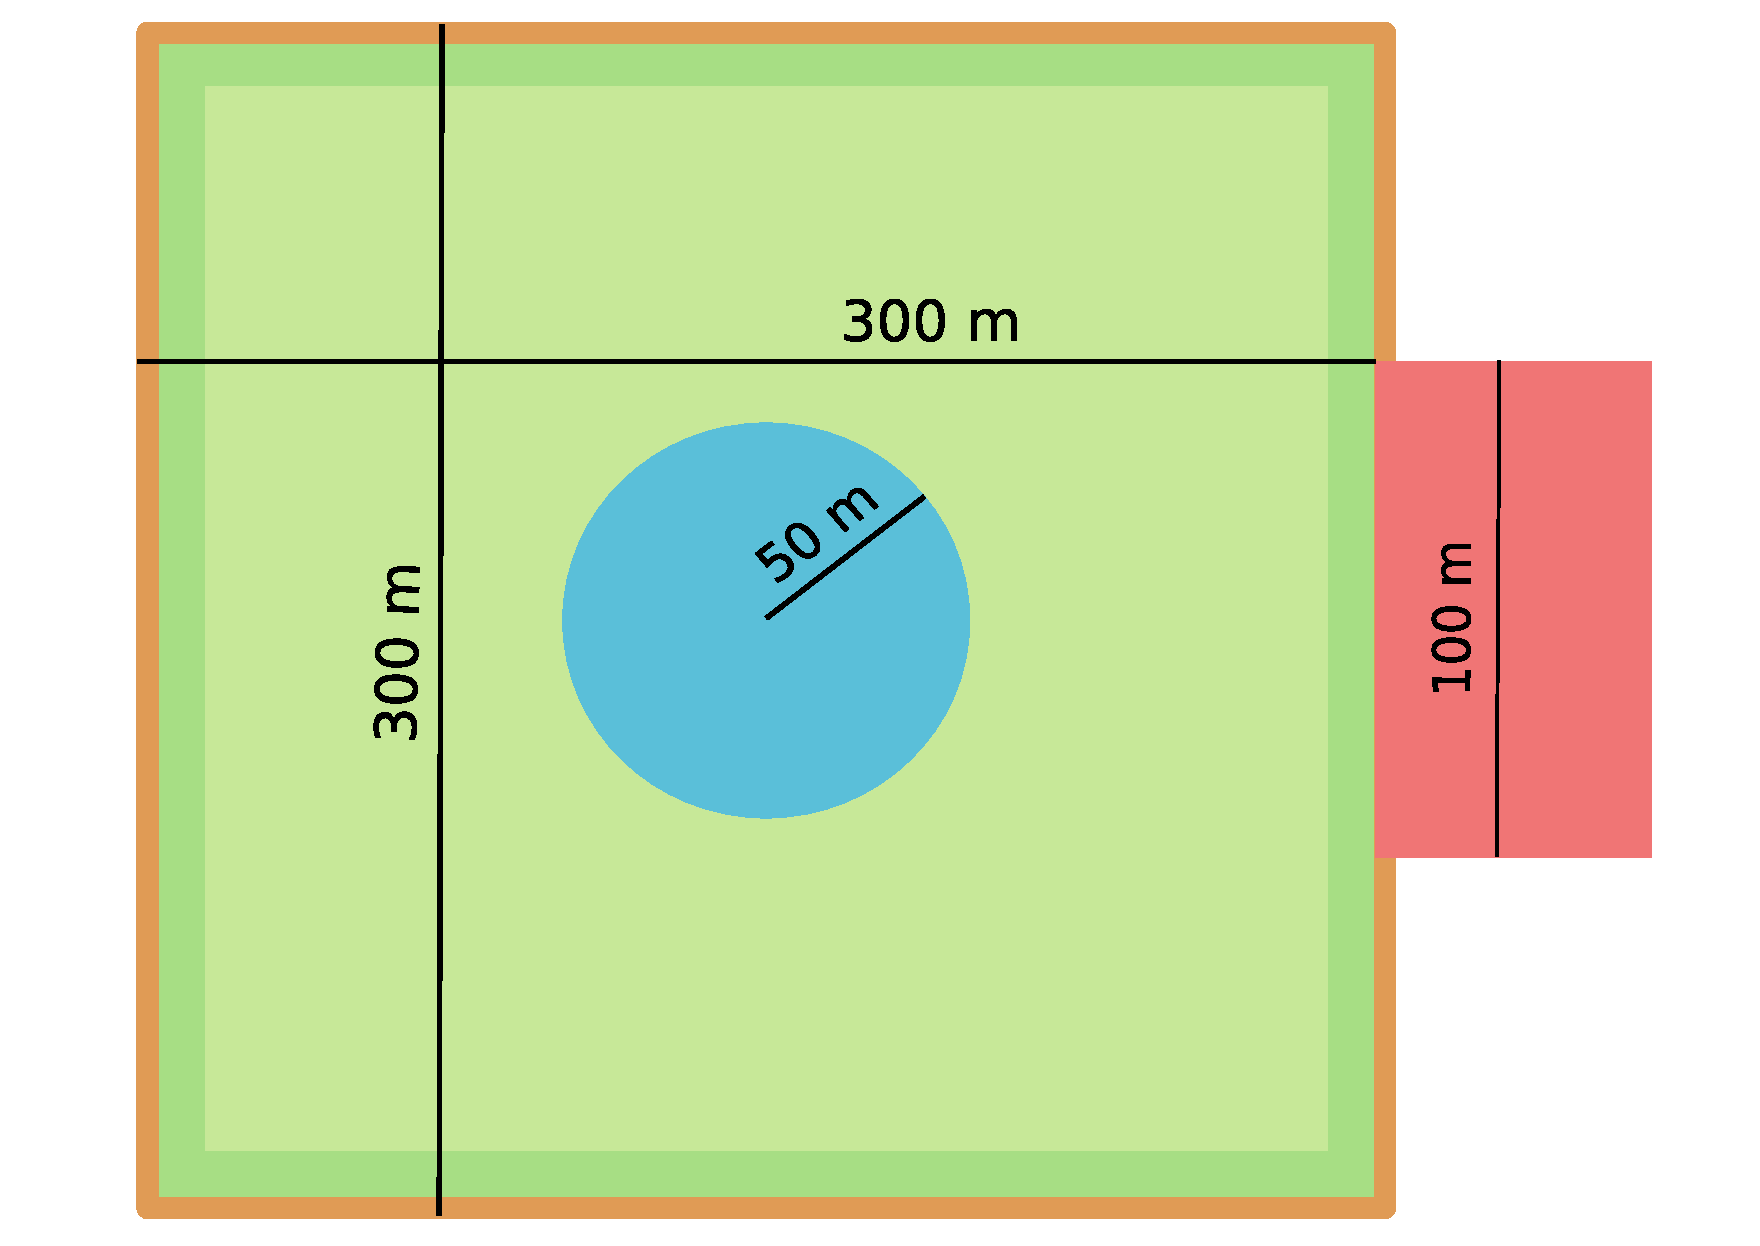
\includegraphics[width=0.7\textwidth]{../poglavja/images/simulacijsko_okolje.pdf}\caption[Območja simulacijskega okolja]{Prikaz območij simulacijskega okolja s pašnikom, stajo in območji porazdelitve agentov.} % narejena je s programom Inkscape
	\label{fig:zemljevid}
\end{figure}

\subsection{Strömbomov model}\label{stroembom}

Prvi in najenostavnejši model gibanja ovc, ki si ga bomo ogledali, temelji na modelu, pri katerem ima vsak agent tri območja, ki ustrezajo trem osnovnim težnjam agenta kot predlagano v~\cite{boids} (slika~\ref{fig:boids}). Osnovne težnje agenta so:
\begin{enumerate}
	\item Agent se od ostalih agentov, ki so mu preblizu, odmika za preprečevanje trkov. Območje odbijanja je izmed vseh najmanjše.
	\item Agent poravna svojo smer gibanja z drugimi agenti, ki so mu dovolj blizu. Območje poravnave je večje od območja odbijanja.
	\item Agent se približuje agentom, ki so v njegovem zaznavnem ali vidnem polju. Območje združevanja je največje.
\end{enumerate}
Od vrste živali je odvisna velikost posameznega območja in moč posamezne težnje. Model je zasnovan za ptice, a ga lahko uporabljamo tudi v ravnini. Str{\"o}mbom je s sodelavci modelu dodal še območje strahu za beg pred grožnjo oziroma ovčarjem in zanemaril območje poravnave. Območje strahu je celo večje od vidnega polja, saj ovca že na daleč psa zazna tudi zaradi njegovega oglašanja, čeprav ta še ni v njenem vidnem polju.

\begin{figure}[ht]  % ali t za na vrhu ali h! za točno tukaj
	\centering
	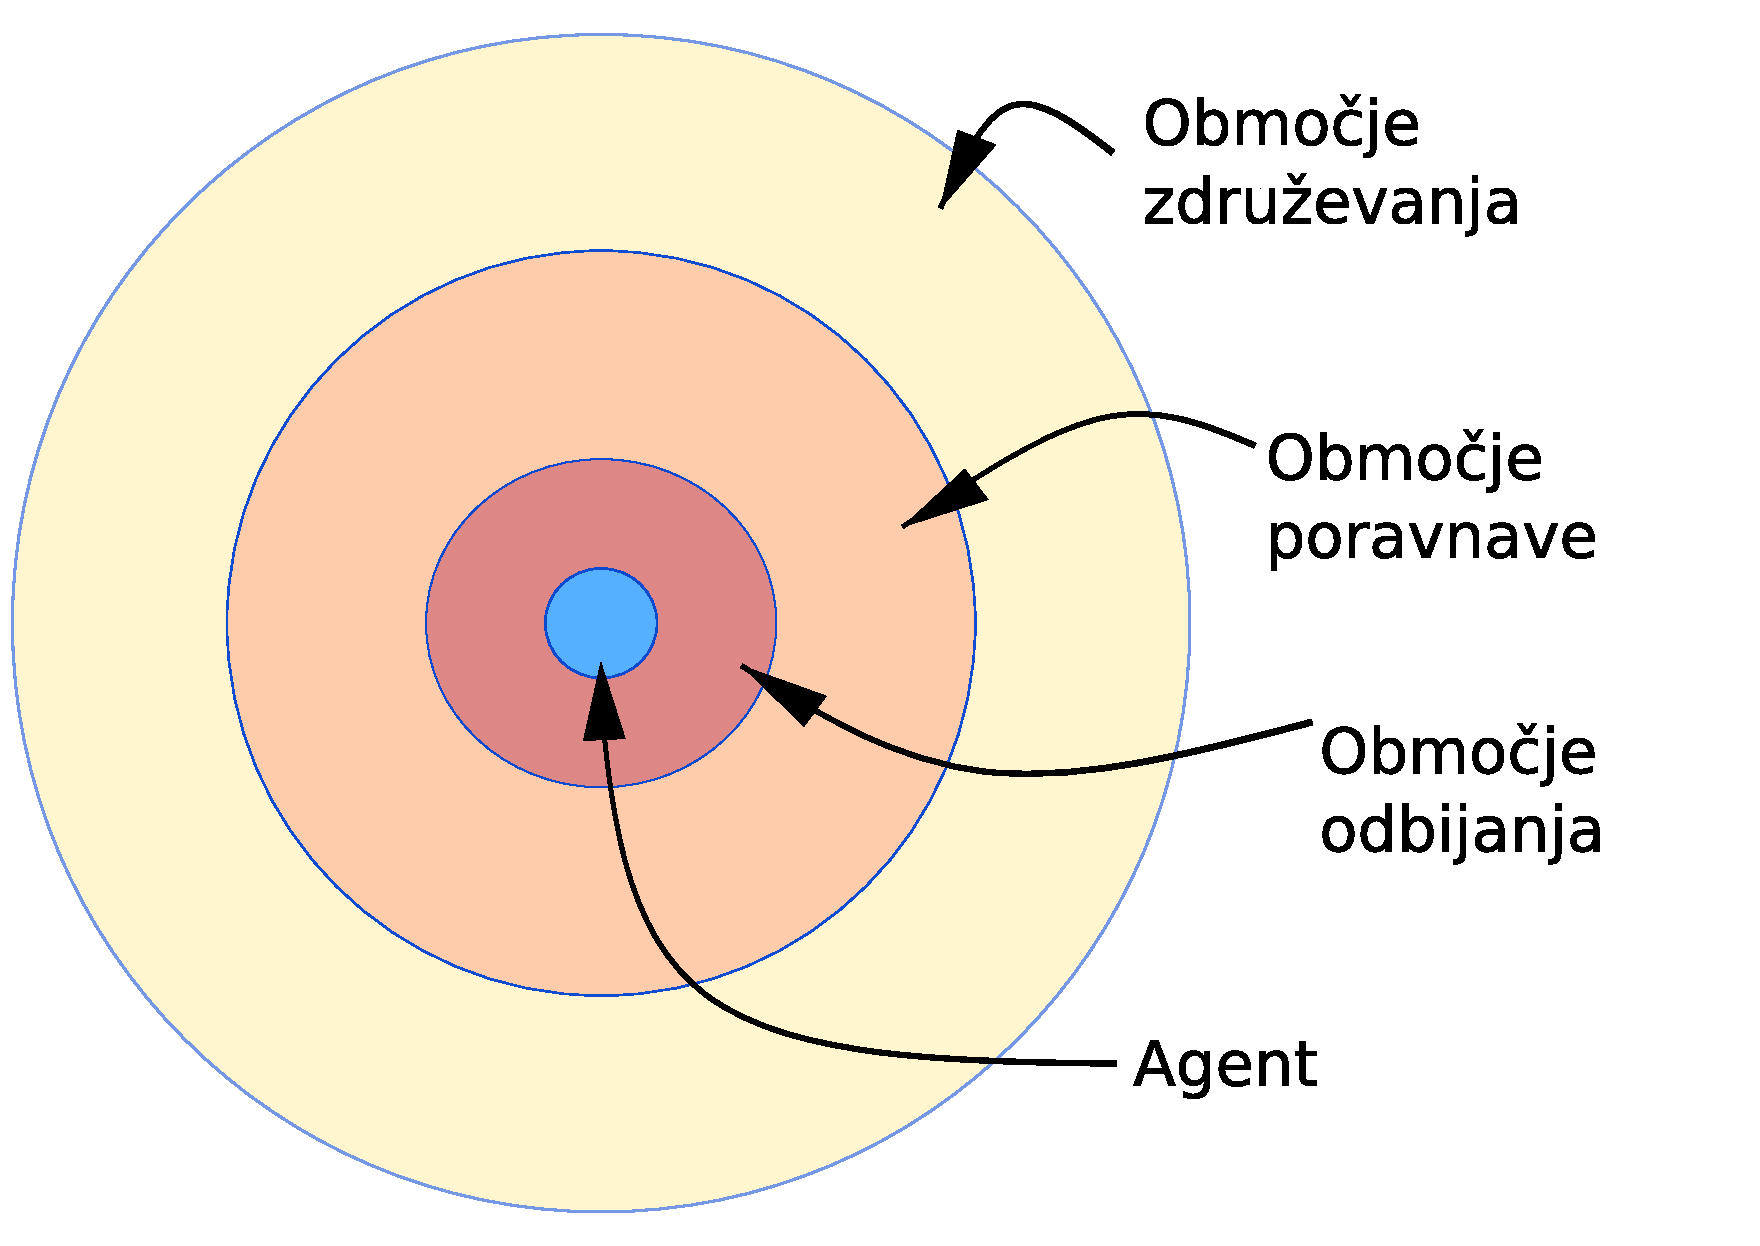
\includegraphics[width=0.7\textwidth]{../poglavja/images/boids.pdf}
	\caption[Območja zaznave]{Prikaz območij modela po~\cite{boids}.} % narejena je s programom Inkscape
	\label{fig:boids}
\end{figure}

\subsubsection{Odbojna sila}

Odbojna sila služi preprečevanju trkov med agenti. Za vsako ovco, ki ima v območju odbijanja vsaj eno ovco, izračunamo odbojno silo $R_i^a$, ki je enaka vsoti normaliziranih vektorjev stran od vsake izmed ovc v območju odbijanja z radijem $r_a$.
\begin{align}
\mathbf{R}_i^a = \sum_{j\not=i,~\Vert \mathbf{A}_i - \mathbf{A}_j\Vert < r_a}\frac{ \mathbf{A}_i - \mathbf{A}_j}{\Vert \mathbf{A}_i - \mathbf{A}_j\Vert}, \label{eq:stroembom-odboj}
\end{align}
kjer je $\mathbf{A}_j$ lokacija $j$-te ovce. Primer si lahko ogledamo na sliki~\ref{fig:stroembom-odboj}.

\begin{figure}[ht]  % ali t za na vrhu ali h! za točno tukaj
	\centering
	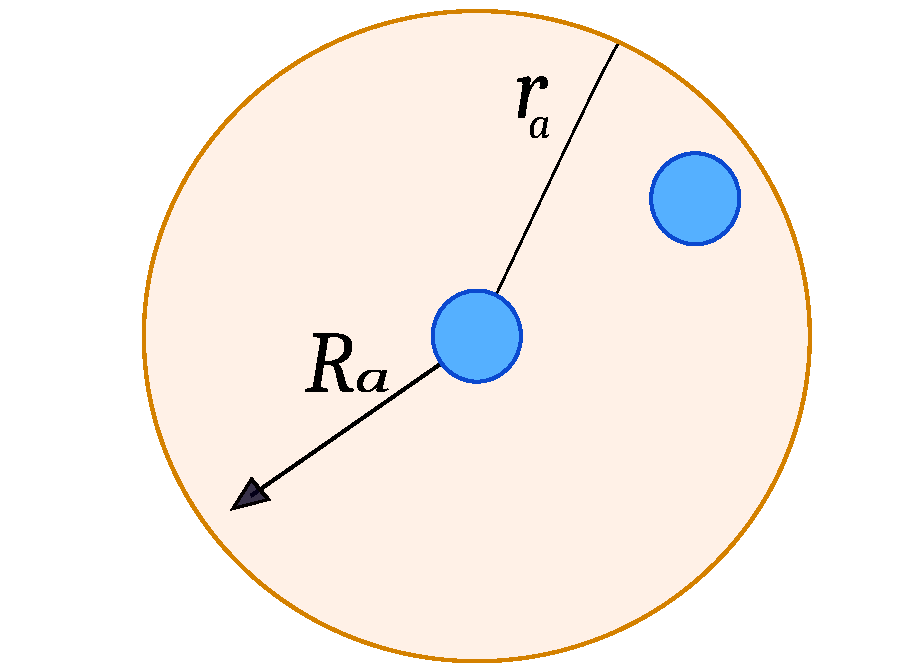
\includegraphics[width=0.49\textwidth]{../poglavja/images/stroembom_odboj.pdf}
	\caption[Odbojna sila]{Odbojna sila od ovce v območju odbijanja.} % narejena je s programom Inkscape
	\label{fig:stroembom-odboj}
\end{figure}

\subsubsection{Sila združevanja}

Ovca želi biti vedno blizu črede, saj se tako počuti varneje. Sila združevanja je kar enaka normaliziranemu vektorju usmerjenemu proti središču dela črede, ki je v njenem vidnem polju oziroma v območju združevanja s polmerom $r_d$, kot je predlagal avtor diplomskega dela~\cite{diplomska}, da bi se izognil situaciji, ko bi se ovce želele približevati ovcam, ki niso v njihovem vidnem polju, saj so avtorji lokalni center izračunavali na podlagi najbližjih $k$ sosedov za nek izbran $k$. V našem primeru pa se lahko zgodi, da ovca vidi vse ali celo nobene druge ovce. Lokalni center mase (LCM) ali lokalno težišče tako izračunamo kot
\begin{align}
\mathbf{LCM}_i = \frac{1}{k}\sum_{\Vert \mathbf{A}_i - \mathbf{A}_j\Vert < r_d} \mathbf{A}_j, \label{eq:stroembom-lcm}
\end{align}
kjer je $k$ število ovc v območju združevanja ovce $i$ vključno z njo samo in se $k$ skozi čas spreminja. Tedaj je smer sile združevanja enaka
\begin{align}
\mathbf{C}_i = \mathbf{LCM}_i - \mathbf{A}_i. \label{eq:stroembom-zdruzi}
\end{align}

Shematski prikaz sile združevanja si lahko ogledamo na sliki~\ref{fig:stroembom-zdruzi}.

\begin{figure}[ht]  % ali t za na vrhu ali h! za točno tukaj
	\centering
	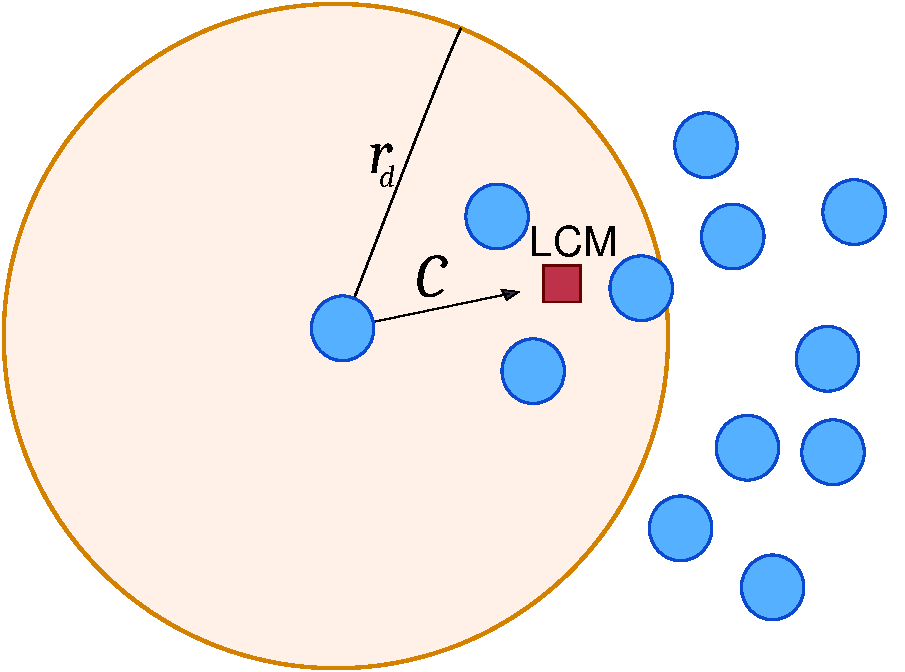
\includegraphics[width=0.49\textwidth]{../poglavja/images/stroembom_zblizevanje.pdf}
	\caption[Sila združevanja]{Sila združevanja v smeri proti lokalnemu centru mase ovc v območju združevanja.} % narejena je s programom Inkscape
	\label{fig:stroembom-zdruzi}
\end{figure}

\subsubsection{Sila bega pred ovčarjem}

Ko ovca zazna grožnjo se želi od nje umakniti. Ovca beži od vseh ovčarjev, ki so v njenem območju bega s polmerom $r_s$. Smer bega izračunamo kot vsoto normaliziranih smeri stran od ovčarjev pomnoženih s faktorjem strahu pred posameznim ovčarjem
\begin{align}
\mathbf{R}_s = \sum_{\Vert \mathbf{A}_i - \mathbf{S}_j\Vert < r_s}\frac{ \mathbf{A}_i - \mathbf{S}_j}{\Vert \mathbf{A}_i - \mathbf{S}_j\Vert}\Big(\frac{ \Vert \mathbf{A}_i - \mathbf{S}_j\Vert - r_s}{r_s}\Big)^2, \label{eq:stroembom-beg}
\end{align}
kjer je $\mathbf{S}_j$ lokacija $j$-tega psa ovčarja. Faktor strahu pred posameznim ovčarjem služi temu, da se ovca bolj boji ovčarja, ki ji je bližje. Za prikaz si oglejmo sliko~\ref{fig:stroembom-beg}.

\begin{figure}[ht]  % ali t za na vrhu ali h! za točno tukaj
	\centering
	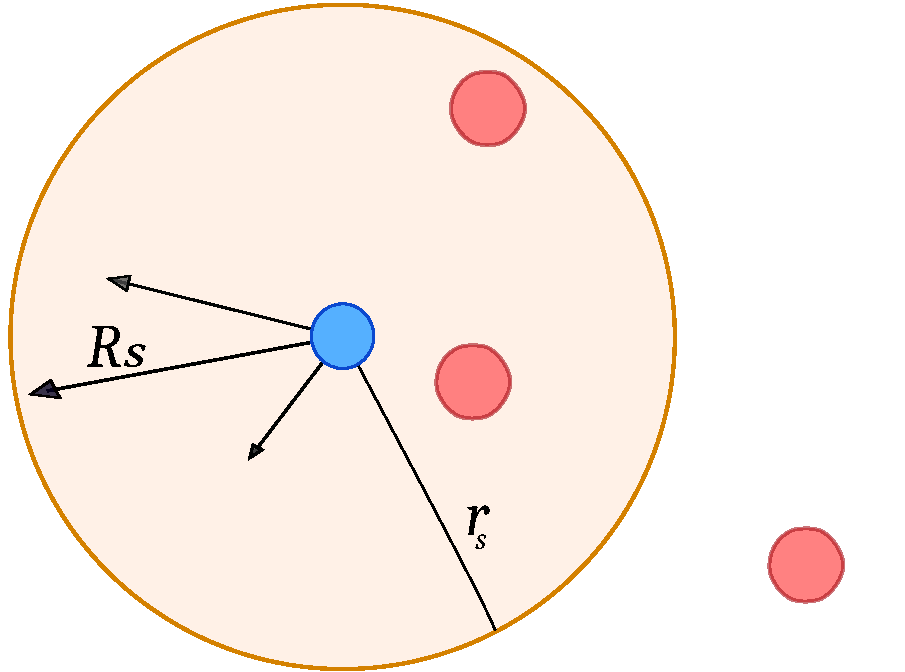
\includegraphics[width=0.49\textwidth]{../poglavja/images/stroembom_beg.pdf}
	\caption[Sila bega pred ovčarjem]{Sila bega pred dvema ovčarjema v območju strahu. Tretji ovčar je ne ogroža.} % narejena je s programom Inkscape
	\label{fig:stroembom-beg}
\end{figure}

\subsubsection{Izračun premika}

Smer gibanja $\mathbf{H}_i^\prime$ izračunamo kot uteženo vsoto vseh izračunanih normaliziranih vektorjev izračunanih po formulah~\eqref{eq:stroembom-odboj}, \eqref{eq:stroembom-zdruzi}, \eqref{eq:stroembom-beg}, normalizirane smeri v prejšnjem koraku $\hat{\mathbf{H}_{i}}$ in naključnega enotskega vektorja $\epsilon$ po formuli
\begin{align}
\mathbf{H}_i^\prime = h\hat{\mathbf{H}_{i}} + c\hat{\mathbf{C}_i} + \rho_a\hat{\mathbf{R}_i^a} + \rho_s\hat{\mathbf{R}_i^s} + e\mathbf{\epsilon}_i, \label{eq:stroembom-smer}
\end{align}
pri čemer izbrane uteži zadoščajo pogoju $\rho_a > c > \rho_s > h > e$, da ovce ostanejo na razdalji in hkrati skupaj kljub grožnji in šumu. Ničelnih vektorjev ne normaliziramo, da se med drugim izognemo begu, ko noben ovčar ni v območju strahu. Stara smer je uporabljena z namenom bolj naravnega gladkega gibanja brez ostrih zavojev. Šum z velikostjo $e$ je prisoten le z verjetnostjo $p$. Agent se ves čas giblje s konstantno hitrostjo $v$. Tako se ovca premakne na točko $\mathbf{A}_i^\prime =\mathbf{A}_i + \Delta t v\hat{\mathbf{H}_i^\prime}$, kjer je $\Delta t$ sprememba časa od prejšnjega koraka in $\hat{\mathbf{H}_i^\prime}$ normalizirana smer izračunana v~\eqref{eq:stroembom-smer}, prilagojena za izogibanje ograji na način, opisan v naslednjem razdelku.

Vrednosti parametrov, ki smo jih uporabili, si lahko ogledamo v tabeli~\ref{table:stroembom}. Večino vrednosti smo povzeli po Str{\"o}mbomu in sodelavcih~\cite{Stroembom} ter Demšarju in sodelavcih~\cite{Demsar}. Zadnja dva parametra nastopata v popravljenem modelu, opisanem v nadaljevanju.

\begin{table}[ht]
	\begin{center}
		\begin{tabular}{ c|l|c }
		\hline
		\textbf{Oznaka} & \textbf{Opis parametra} & \textbf{Uporabljena vrednost} \\ \hline  
		$r_a$ & Polmer območja odbijanja & 2~m \\ 
		$r_s$ & Polmer območja združevanja & 30~m \\ 
		$r_d$ & Polmer območja strahu & 15~m \\ 
		$\rho_a$ & Relativna moč odbojne sile & 2 \\ 
		$c$ & Relativna moč sile združevanja & 1,05 \\ 
		$\rho_s$ & Relativna moč sile bega pred ovčarjem & 1 \\ 
		$h$ & Relativna moč prejšnje smeri & 0,5 \\ 
		$e$ & Relativna moč šuma & 0,3 \\ 
		$p$ & Verjetnost nastanka šuma & 0,05 \\ 
		$v$ & Hitrost premikanja & 5~m/s \\ 
		$r_f$ & Razdalja za izogibanje ograji & 20~m \\ 
		$\gamma$ & Stopnja izogibanja ograji & 0,01 \\ \hline
		$v_p$ & Hitrost premikanja v odsotnosti grožnje & 0,5~m/s \\ 
		$\phi$ & Faktor dovoljene spremembe smeri & $\pi / 20$~rad \\ 
		\hline
		\end{tabular}
	\end{center}
\caption[Parametri Str{\"o}mbomovega modela gibanja ovc]{Parametri Str{\"o}mbomovega modela. Spodnja dva parametra potrebujemo samo za popravljen Str{\"o}mbomov model opisan v poglavju~\ref{popravljen}.}
\label{table:stroembom}
\end{table}

\subsubsection{Izogibanje ograji}\label{ograja}

Ovca se od vsakega dela ograje, ki ji je bliže od $r_f$, želi odmakniti. Smeri $\hat{\mathbf{H}_i^\prime}$ zato prištejemo odbojno silo v smeri stran od ograje z velikostjo $\gamma (r_f - d_{i,j}) / r_f$, kjer je $\gamma$ stopnja izogibanja ograji in $d_{i,j}$ oddaljenost $i$-te ovce do $j$-tega dela ograje, kakor so predlagali Demšar in sodelavci~\cite{Demsar}. Smer gibanja ponovno normaliziramo.

\subsection{Popravljen Strömbomov model}\label{popravljen}

Ovce se po opisanem Str{\"o}mbomovem modelu ne gibljejo najbolj naravno. Oblikujejo se manjše črede, ki se združijo, ko so dovolj blizu in izgledajo bolj podobne kapljam olja na vodi kakor pa čredi ovc (slika~\ref{fig:stroembom-olje}). Čreda ima kristalno in pretirano strukturirano obliko, saj ovce striktno ohranjajo določeno medsebojno razdaljo, ko so si enkrat dovolj blizu. Ker pa se ne bi smele premikati za ohranjanje te razdalje, se le tresejo okrog svoje osi. Ta problem smo rešili z določanjem največjega dovoljenega kota spremembe smeri v časovnem koraku. Največji dovoljen kot definiramo kot $\phi_v = \phi / \sqrt{v_t}$, kjer je $\phi$ faktor največje dovoljene spremembe smeri in $v_t$ trenutna hitrost. Večja kot je trenutna hitrost, manjše spremembe smeri dovolimo. Velikost spremembe smeri omejimo s $\phi_v$. Tako ovci stabiliziramo smer gibanja po tem, ko je nova smer izračunana. Na ta način smo rešili problem med begom, saj gredo vse ovce v podobno smer z manj tresenja.

Ker pa so ovce ob tej fiksni hitrosti in majhnem dovoljenem kotu začele krožiti kot roj mušic, kadar grožnja ni bila prisotna, in je čreda zato obstala na mestu, smo uvedli spremenljivko $v_t$, ki predstavlja trenutno hitrost. Ovca se zdaj giblje s hitrostjo enako $v_t = \frac{3}{10}v_z + \frac{7}{10}v_{t-1}$, kjer je $v_{t-1}$ hitrost v prejšnjem koraku in $v_z$ želena hitrost, ki je enaka $v$ v času prisotne grožnje in $v_p$ sicer med pašo. Tako se ovca v času odsotnosti grožnje premika počasneje in ne začne krožiti, gibanje pa postane bolj naravno. Prednost dodatnega modela je predvsem v tem, da je dovolj drugačen od ostalih dveh opisanih v poglavjih~\ref{stroembom} in \ref{ginelli}. Tako bomo lahko testirali robustnost pristopa vodenja s psi ovčarji za primer, ko bi želeli voditi drugačno vrsto agentov (živali, ljudi ali delcev).

Že Str{\"o}mbomov model smo nekoliko spremenili, maš model mu ni več pretirano podoben, ampak ga vseeno imenujmo \textit{Popravljen Str{\"o}mbomov model}, saj smo ohranili osnovno idejo. Čeprav je tu gibanje bolj naravno kot v osnovnem modelu, pa ni dovolj podobno realnemu gibanju ovc.

\begin{figure}[ht]  % ali t za na vrhu ali h! za točno tukaj
	\centering
	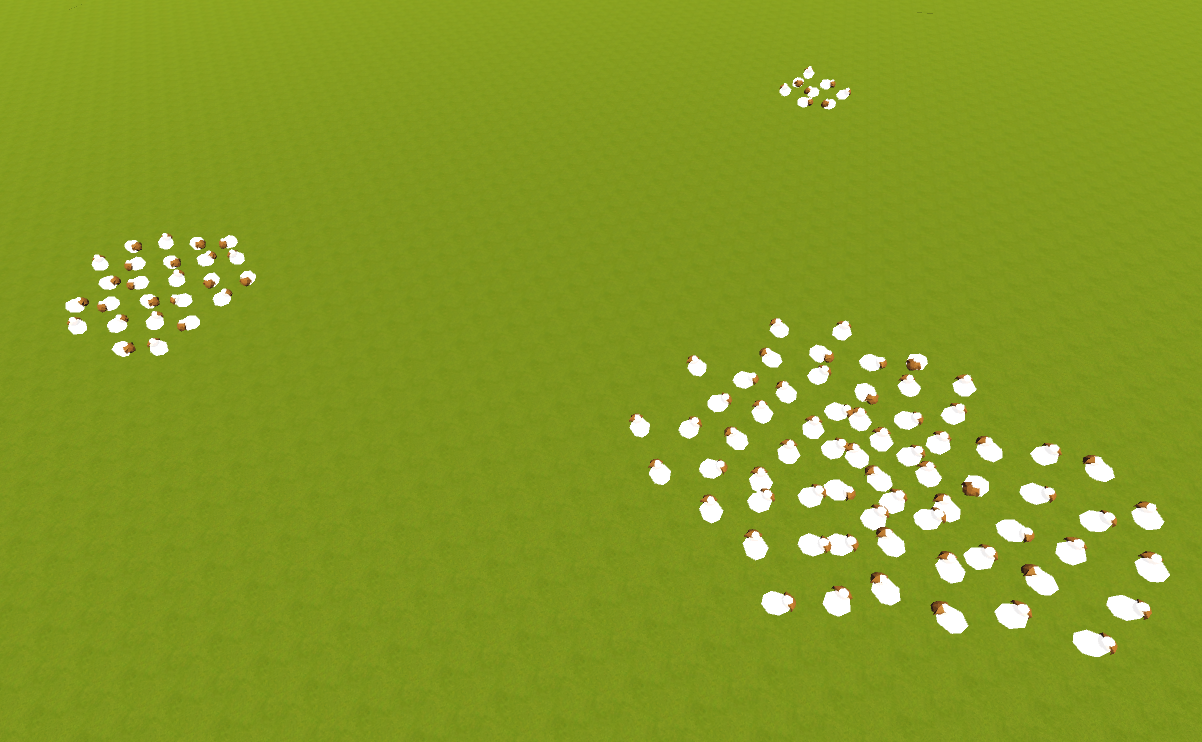
\includegraphics[width=0.52\textwidth]{../poglavja/images/stroembom-creda.png}
	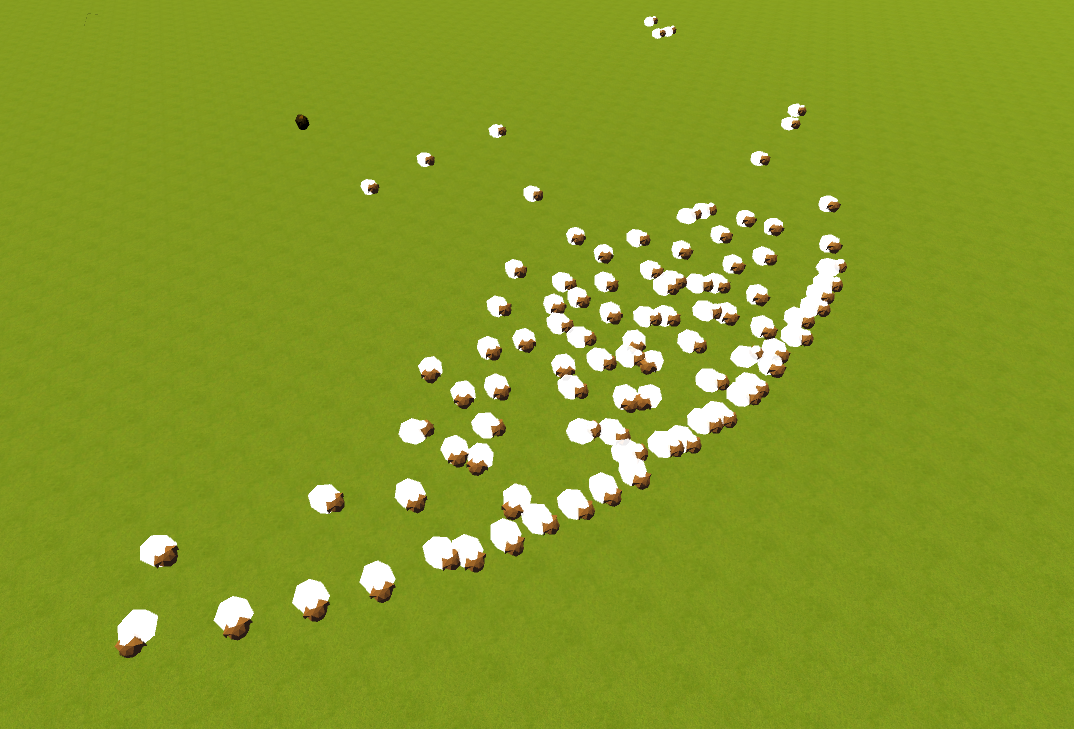
\includegraphics[width=0.47\textwidth]{../poglavja/images/popravljen-stroembom-creda.png}
	
	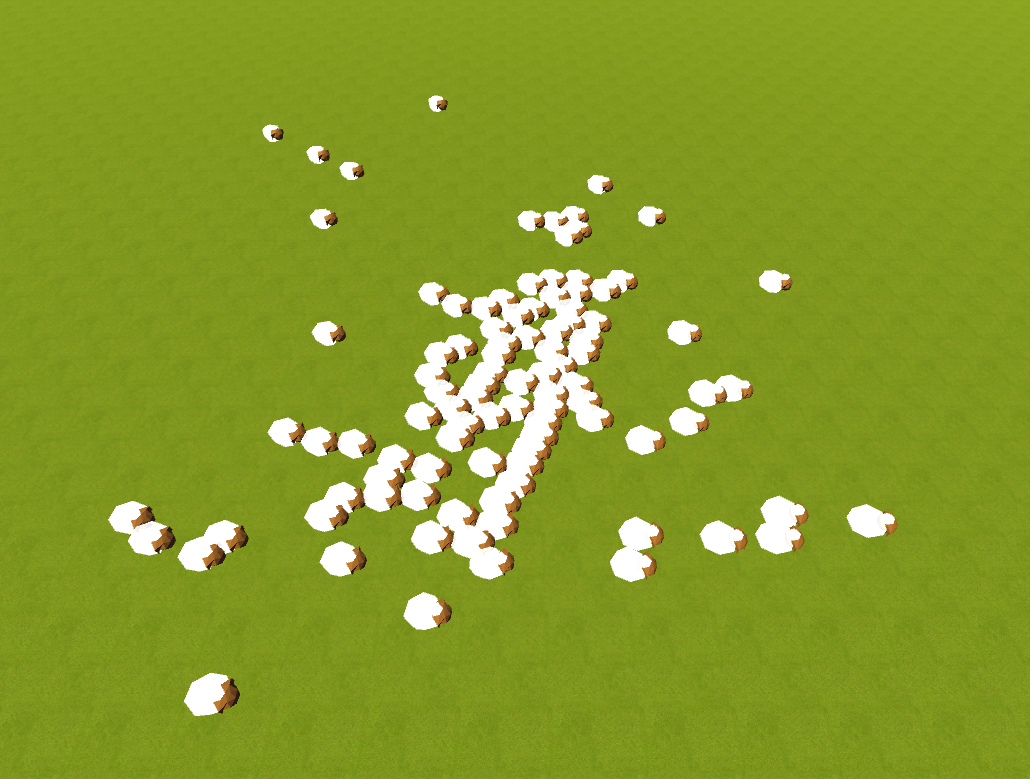
\includegraphics[width=0.49\textwidth]{../poglavja/images/ginelli-creda.png}
	\caption[Struktura črede po vseh treh modelih]{Levo zgoraj vidimo značilno kristalno strukturo črede po Str{\"o}mbomovem modelu, ki se ohranja celo med begom pred ovčarjem. Desno zgoraj opazimo nekoliko bolj naravno strukturo pri popravljenem Str{\"o}mbomovem modelu. Ovce se po popravljenem modelu gibljejo bolj naravno, a ne dovolj podobno realnemu gibanju ovc v naravi. Na spodnji sliki je primer črede med begom v primeru Ginellijevega modela. Gre za naprednejši model, osnovan na dejanskih podatkih o gibanju ovc iz narave. Ta model je opisan v naslednjem podpoglavju.} % narejena je s programom Inkscape
	\label{fig:stroembom-olje}
\end{figure}

\subsection{Ginellijev model}\label{ginelli}

Osnovni Str{\"o}mbomov model ima določene pomanjkljivosti, saj so ovce ves čas preveč oddaljene in se bolj ne približajo druga drugi niti med begom, kar pa se v naravi navadno ne zgodi. Str{\"o}mbomov model ne temelji na posnemanju dejanskega gibanja ovc, ampak je le enostaven model za testiranje njihove ideje vodenja psa ovčarja. V članku avtorji namreč predstavijo model vodenja psa ovčarja, ki si ga bomo ogledali v naslednjem poglavju ter mu dodali nekaj izboljšav.

Ginelli je s sodelavci v svojem članku~\cite{Ginelli} opisal bolj kompleksen model gibanja ovc, ki so ga razvili in testirali z eksperimentalnimi posnetki črede ovc v kvadratni ogradi in so se s tem bolj približali dejanskemu obnašanju ovc. Opazili so nekakšno utripanje črede. Čreda se je ponavljajoče širila po pašniku in se ob naključnem času na hitro zbrala tudi brez prisotnosti grožnje. S tem so ovce hkrati popasle večje območje in ostale varno skupaj. Vsaka ovca je imela vedno več prostora, dokler ni kakšna ovca ob robu stekla proti notranjosti črede, kar je s črednim nagonom povzročilo tek večine ovc in so se tako hitro zbrale ter nekoliko premaknile center črede. Ta model pa za razliko od Str{\"o}mbomovega modela upošteva poleg lokacije ovc $\mathbf{A}_i^t$ tudi njihovo smer $\Theta^t$ in stanje obnašanja $q_i^t$. Stanja obnašanja so mirovanje, hoja in tek, ki jih označimo kot 0, 1 in 2. Ovca med mirovanjem ne spreminja lokacije in smeri, sicer pa ju prilagaja glede na bližnje ovce.

\subsubsection{Izračun smeri}

Agent se premakne po enačbi
\begin{align}
\mathbf{A}_i^{t+\Delta t} &= \mathbf{A}_i^t + \Delta tv(q_i^t)\mathbf{s}_i^{t+\Delta t}, \label{eq:ginelli-premik}
\end{align}
kjer je $\Delta t$ sprememba časa med korakoma simulacije, hitrost je zdaj odvisna od stanja v prejšnjem koraku in smernega vektorja $\mathbf{s}_i^t = (cos\Theta_i^t, sin\Theta_i^t)$, odvisnega od trenutnega kota $\Theta_i^t$. Ob tem upoštevamo, da je hitrost v stanju teka $v(2)$ veliko večja od hitrosti med hojo $v(1)$, ki pa je večja od 0. Torej velja $v(2) >> v(1) > v(0) = 0$.

Ovca želi svojo smer poravnati s smerjo drugih ovc, ki so od nje oddaljene največ $r_o$, po enačbi
\begin{align}
\Theta_i^{t+\Delta t} &= Arg\lbrack\sum_{j\not=i,~\Vert \mathbf{A}_i^t - \mathbf{A}_j^t\Vert < r_o}s_j^t\rbrack+\psi_i^t, \label{eq:ginelli-hoja}
\end{align}
kjer je $Arg$ argument vektorja oziroma kot od baznega vektorja in $\psi_i^t$ naključen kot z intervala $\lbrack-\mu\pi,\mu\pi\rbrack$. S tem smo dobili povprečno smer okoliških ovc z nekaj šuma. V stanju teka pa je ovca pozorna le na ovce, ki so prav tako v stanju teka in so največ $r_d$ oddaljene od nje. Pri tem upošteva njihovo smer gibanja, razdaljo do njih in v kateri smeri so. V stanju teka se smer gibanja izračunava na sledeč način:
\begin{align}
\Theta_i^{t+\Delta t} &= Arg\lbrack\sum_{j\in \mathcal{V}_i}(\delta \mathbf{s}_j^t+\beta f(r_{i,j}^t)\mathbf{e}_{i,j}^t)\rbrack, \label{eq:ginelli-tek}
\end{align}
kjer je $\mathcal{V}_i = \lbrace j\not=i,~\Vert \mathbf{A}_i^t - \mathbf{A}_j^t\Vert < r_d,~q_j^t=2\rbrace$ množica vseh okoliških ovc v stanju teka, $\delta$ utež posnemanja smeri okoliških ovc, $\mathbf{e}_{i,j}^t$ enotski vektor od $i$-te do $j$-te ovce z utežjo $\beta$ in $f(r_{i,j}^t)$ faktor privlačno-odbojne sile z ravnovesno razdaljo $r_e$, odvisen od razdalje med $i$-to in $j$-to ovco. Ta faktor je od razdalje $r$ odvisen na sledeč način:
\begin{align}
f(r) &= min(1, \frac{r-r_e}{r_e}). \label{eq:ginelli-faktor}
\end{align}
To povzroči, da se ovca približa ostalim ovcam na udobno razdaljo $r_e$ in teče v isti smeri kot one. Zaradi poravnave z bližnjo okolico se ob večji gneči ovce postavijo v vrste, kar so za podobne primere že dokazali avtorji članka~\cite{degond2015continuum}, kjer matematično modelirajo obnašanje podolgovatih delcev, ki se zaradi tresenja in posledičnih trkov z bližnjimi delci poravnajo z njimi. Ovca smer še dodatno spremeni v bližini ograje na enak način kot v ostalih dveh modelih gibanja ovc, kakor smo opisali v poglavju~\ref{ograja} na strani~\pageref{ograja}.

Vrednosti parametrov, ki smo jih uporabili za ta model, si lahko ogledamo v tabeli~\ref{table:ginelli}. Večino vrednosti so predlagali avtorji člankov~\cite{Ginelli} in \cite{Demsar}.

\begin{table}[ht]
	\begin{center}
		\begin{tabular}{ c|l|c }
			\hline
			\textbf{Oznaka} & \textbf{Opis parametra} & \textbf{Uporabljena vrednost} \\ \hline  
			$v(1)$ & Hitrost hoje & 0,5~m/s \\ 
			$v(2)$ & Hitrost teka & 5~m/s \\ 
			$\tau_{0\rightarrow1}$ & Stopnja prehoda iz mirovanja v hojo & 70 \\ 
			$\tau_{1\rightarrow0}$ & Stopnja prehoda iz hoje v mirovanje & 16 \\ 
			$\tau_{0,1\rightarrow2}$ & Stopnja prehoda v tek & $N$ \\ 
			$\tau_{2\rightarrow0}$ & Stopnja prehoda iz teka v mirovanje & $N$ \\ 
			$d_R$ & Utež prehoda v tek & 31,6 \\ 
			$d_S$ & Utež prehoda iz teka & 2,1 \\ 
			$r_e$ & Ravnovesna razdalja med ovcami & 1~m \\ 
			$r_o$ & Razdalja za poravnavo z ovcami med hojo & 1~m \\ 
			$r_d$ & Razdalja za poravnavo med tekom & 15~m \\ 
			$r_s$ & Razdalja za zaznavo psa ovčarja & 30~m \\
			$\alpha$ & Utež intenzivnosti oponašanja & 15 \\ 
			$\beta$ & Moč privlačno-odbojne sile & 0,8 \\ 
			$\delta$ & Moč poravnave med tekom & 4 \\ 
			$\mu$ & Razpon šuma & 0,13 \\ 
			$\gamma$ & Moč strahu pred ovčarjem & 0,1 \\ 
			\hline
		\end{tabular}
	\end{center}
	\caption[Parametri Ginellijevega modela gibanja ovc]{Parametri Ginellijevega modela, kjer je $N$ število ovc.}
	\label{table:ginelli}
\end{table}

\subsubsection{Sprememba stanja obnašanja}

Ovca spremeni svoje stanje obnašanja $q_i^t$ glede na okoliške ovce in grožnje. Ovca z večjo verjetnostjo preklopi v neko stanje, če je v njeni okolici več ovc v tem izbranem stanju. Definirajmo verjetnost prehoda iz mirovanja v hojo $p_{0\rightarrow1}$ in verjetnost prehoda iz hoje v mirovanje $p_{1\rightarrow0}$ za ovco $i$ ob času $t$ na podoben način
\begin{align}
p_{a\rightarrow b}(i, t)=1 - exp(-\frac{1+\alpha n_b^t(i)}{\tau_{a\rightarrow b}}), \label{eq:stanje-hoja}
\end{align}
kjer je $\alpha$ utež intenzivnosti obnašanja, $n_b^t(i)$ število ovc v stanju gibanja $b$ ob času t v okolici ovce $i$, oddaljenih največ $r_d$, in $\tau_{a\rightarrow b}$ stopnja prehoda iz stanja $a$ v stanje $b$.

Avtorji so model poenostavili s tem, da je verjetnost prehoda iz mirovanja ali hoje v tek enaka in da ovca iz stanja teka vedno najprej preide v stanje mirovanja. Definirajmo še ti dve verjetnosti.
Verjetnost prehoda iz mirovanja ali hoje v tek je enaka
\begin{align}
p_{0,1\rightarrow2}(i, t)=1 - exp(-\frac{1}{\tau_{0,1\rightarrow 2}}\lbrack \frac{l_i^t}{d_R}(1+\alpha m_R^t(i))\rbrack^\delta), \label{eq:v-tek}
\end{align}
kjer je $\tau_{0,1\rightarrow 2}$ stopnja prehoda v tek, $l_i^t$ povprečna razdalja do metrično sosednjih ovc, $d_R$ utež prehoda v tek, $m_R^t$ število metrično sosednjih ovc v stanju teka in $\delta>0$ moč poravnave med tekom. Ovca je metrično sosednja, če je na prvi Voronoievi lupini. S tem bolj razkropljena čreda prične teči z večjo verjetnostjo kot manj razpršena zaradi vpliva $l_i^t$, pozitiven $\delta$ pa poskrbi za konveksen vpliv razpršenosti na pričetek teka. Ovca se v stanju teka ustavi z verjetnostjo
\begin{align}
p_{2\rightarrow0}(i, t)=1 - exp(-\frac{1}{\tau_{2\rightarrow 0}}\lbrack \frac{d_S}{l_i^t}(1+\alpha m_S^t(i))\rbrack^\delta), \label{eq:iz-teka}
\end{align}
kjer je $\tau_{2\rightarrow 0}$ stopnja prehoda iz teka v mirovanje, $d_S$ utež prehoda iz teka in $m_S^t(i)$ število metrično sosednjih ustavljajočih se ovc. Opazimo, da ima tu povprečna razdalja do sosedov obraten vpliv kot v enačbi~\eqref{eq:v-tek}.
Shemo sprememb stanj si lahko ogledamo na sliki~\ref{fig:ginelli-stanja}.

\begin{figure}[ht]  % ali t za na vrhu ali h! za točno tukaj
	\centering
	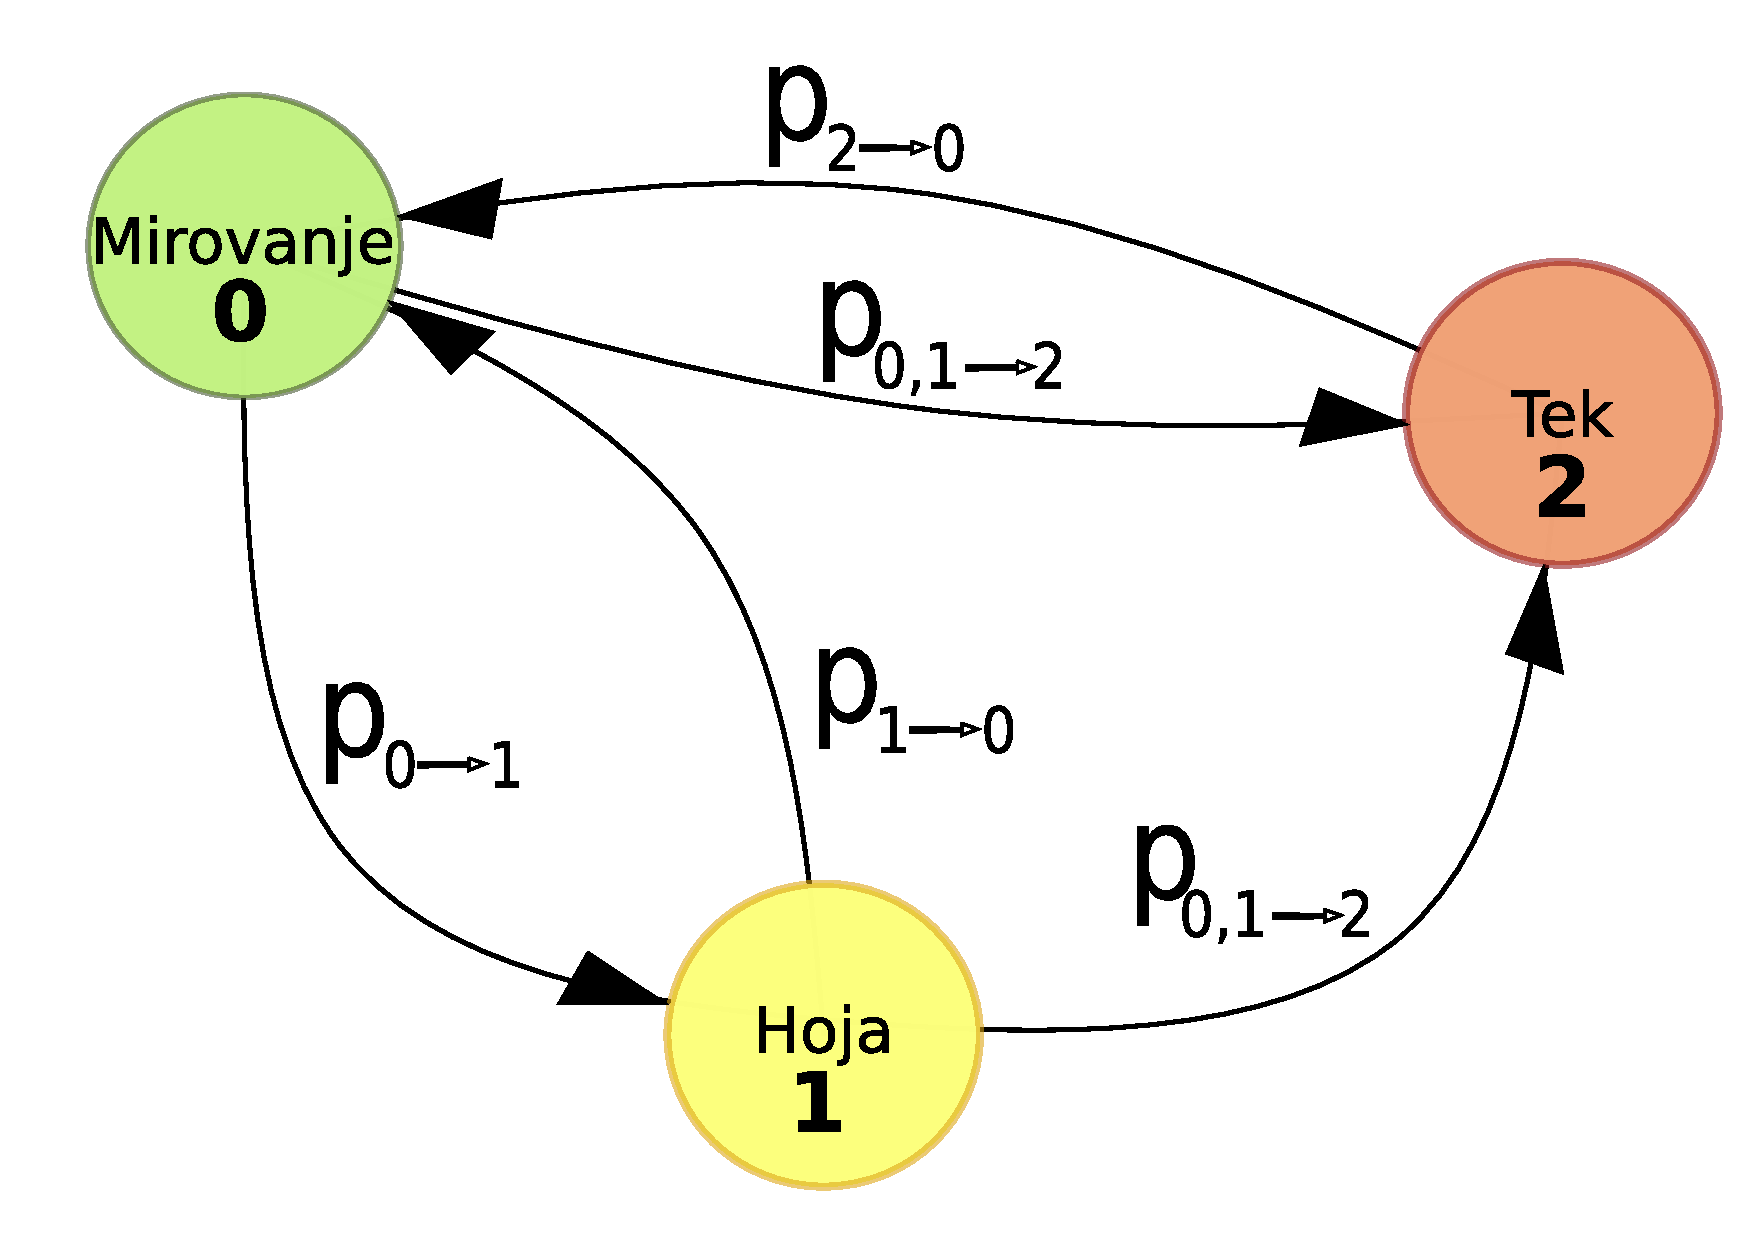
\includegraphics[width=0.6\textwidth]{../poglavja/images/prehodi.pdf}
	\caption[Možni prehodi med stanji gibanja]{Možni prehodi med stanji gibanja.} % narejena je s programom Inkscape
	\label{fig:ginelli-stanja}
\end{figure}

\subsubsection{Beg pred ovčarjem}

Ker se izvirni članek ne ukvarja z vodenjem črede, njihov model ne vsebuje odziva na prisotnost grožnje. Za naše potrebe smo modelu gibanja ovce dodali strah pred ovčarjem. Že pri Str{\"o}mbomovem modelu smo pri tem upoštevali možnost vodenja z več psi ovčarji.

Ovca naj gre v primeru prisotnosti grožnje na razdalji največ $r_s$ vedno v stanje teka. Smer bega pred ovčarji v primeru njegove prisotnosti določimo kot
\begin{align}
\Theta_i^t&=Arg\lbrack \hat{\mathbf{s}}_i^t+\gamma\hat{\mathbf{R}_s}\rbrack,\label{eq:ginelli-beg}
\end{align}
kjer je $\hat{\mathbf{s}}_i^t$ normiran smerni vektor s kotom, izračunanim po enačbi~\eqref{eq:ginelli-tek}, $\gamma$ moč strahu pred ovčarjem in $\hat{\mathbf{R}_s}$ normirana sila bega, izračunana enako kot za Str{\"o}mbomov model v enačbi~\eqref{eq:stroembom-beg}. Ovco je tako bolj strah bližje grožnje, a ji je smer bega celotne črede bolj pomembna kot smer ovčarja.
